\documentclass[dvipsnames, 10pt]{beamer}
%%%
% PREAMBLE FOR THIS DOC 
%%%
%https://tex.stackexchange.com/questions/68821/is-it-possible-to-create-a-latex-preamble-header
\usepackage{/Users/miw267/Repos/latex_preamble/beamer_preamble}


%%%
% DOCUMENT
%%%

\begin{document}



\title{09/11/2026: Lists}
\author{CSCI 246: Discrete Structures}
\date{Textbook reference: Sec. 8, Scheinerman}

\begin{frame}
    \titlepage 
\end{frame}


%\begin{frame}
%\footnotesize 
%
%\begin{mygreenbox}[title=Graded Quiz Pickup]
%Quizzes are in the front of the room, grouped into four bins (A-G, H-L, M-R, S-Z) by last name. The quizzes are upside down with your last name on the back. Come find yours before, during, or after class.  Only turn the quiz over if it's yours.
%\end{mygreenbox} 
%\vfill 
%
%\begin{myredbox}[title=Announcements]
%
%\begin{itemize}
%\item Friday's problems quiz will cover \textbf{Boolean Algebra} and \textbf{Induction}.
%\item The handwritten scores on Friday's quizzes were presented out of five points TOTAL (2.5 points per problem), but the histograms I showed last class were out of five points per each question.   
%\end{itemize}
%
%\end{myredbox}
%
%\vfill 
%
%
%\begin{myyellowbox}[title=Today's Agenda]
%\begin{itemize}
%	\item Reading quiz  (5 mins)
%	\item Mini-lecture ($\approx$ 20 mins)
%	%
%	\begin{itemize}
%	\footnotesize 
%	\item Review induction 
%	\end{itemize}
%	%
%	\item Group exercises ($\approx$ 20 mins)
%\end{itemize}
%
%\end{myyellowbox}
%\vfill 
%
%\end{frame}





\begin{frame}

\vfill 
\begin{myredbox}[title=Announcements]
\begin{itemize}
	\item Early-access version of the slides should are posted to the course repo before class starts. (The early-access version will not yet contain the group exercises or, if relevant, a quiz).
	\item The full version of the slides are posted to the course repo after class ends. \textbf{Starting today, the full slide deck will be posted to the repo \emph{automatically} at 3pm.}
\end{itemize}
\end{myredbox} 
\vfill 

\begin{myyellowbox}[title=Today's Agenda]
\begin{itemize}
	\item Quiz ($\approx$ 15 mins)
	\item Review of Boolean Algebra ($\approx$ 10 mins)
	\item Mini-lecture: Lists ($\approx$ 10 mins)
	\item Group exercises ($\approx$ 10 mins)
\end{itemize}

\end{myyellowbox}
\end{frame}






\begin{frame}{Poll}

\begin{center}
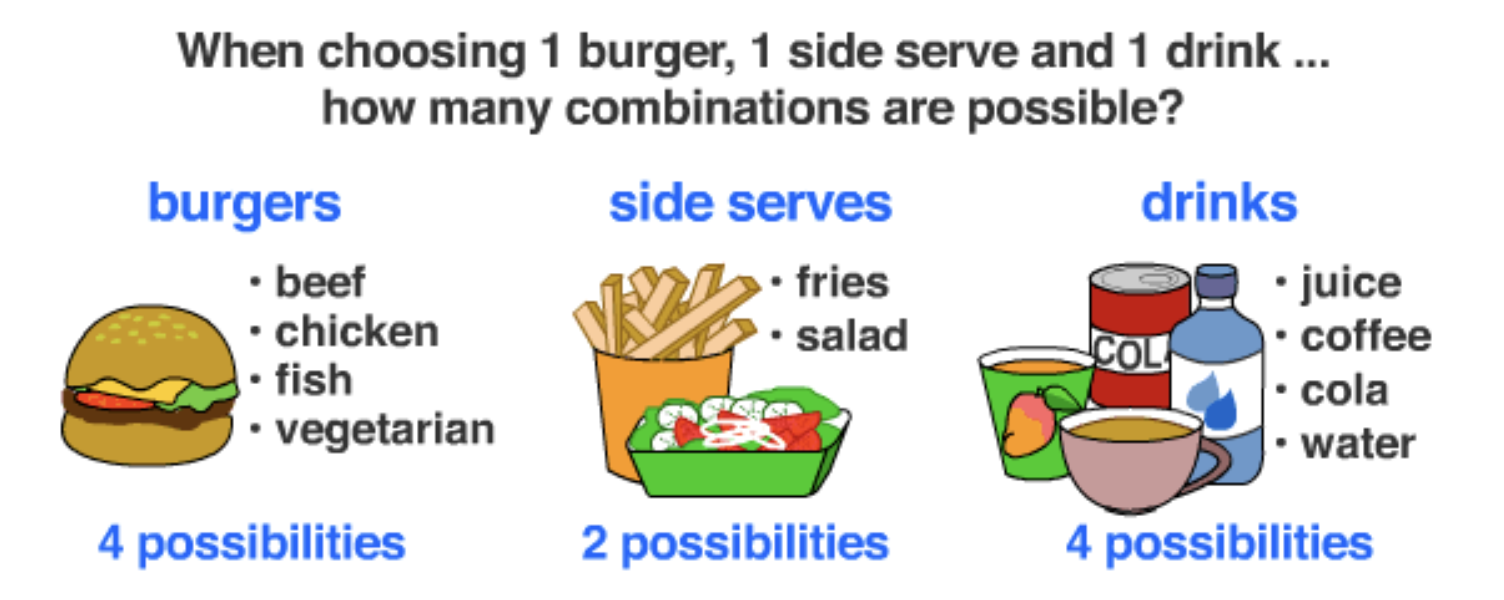
\includegraphics[width=\textwidth]{images/multiplication_principle.png}
\pause \vfill 
\Large \colorbox{blue!30}{\textbf{Solution.}} \blue{There are $4 \times 2 \times 4 = 32$ possibilities.}
\end{center}


\end{frame}



\begin{frame}{Lists}

\begin{mygreenbox}[title=Definition]
A \textbf{list} is an ordered sequence of objects.
\end{mygreenbox}

\pause \vfill 

\colorbox{yellow!30}{\textbf{Example}: All possible meal combinations for the fast food problem}
\small
\begin{columns}[t]
  \begin{column}{0.25\textwidth}
    \begin{tabular}{l}
      (beef, fries, juice) \\
      (beef, fries, coffee) \\
      (beef, fries, cola) \\
      (beef, fries, water) \\
      \\
      (beef, salad, juice) \\
      (beef, salad, coffee) \\
      (beef, salad, cola) \\
      (beef, salad, water) \\
    \end{tabular}
  \end{column}

  \begin{column}{0.28\textwidth}
    \begin{tabular}{l}
      (chicken, fries, juice) \\
      (chicken, fries, coffee) \\
      (chicken, fries, cola) \\
      (chicken, fries, water) \\
      \\
      (chicken, salad, juice) \\
      (chicken, salad, coffee) \\
      (chicken, salad, cola) \\
      (chicken, salad, water) \\
    \end{tabular}
  \end{column}

  \begin{column}{0.22\textwidth}
    \begin{tabular}{l}
      (fish, fries, juice) \\
      (fish, fries, coffee) \\
      (fish, fries, cola) \\
      (fish, fries, water) \\
      \\
      (fish, salad, juice) \\
      (fish, salad, coffee) \\
      (fish, salad, cola) \\
      (fish, salad, water) \\
    \end{tabular}
  \end{column}

  \begin{column}{0.25\textwidth}
    \begin{tabular}{l}
      (veg, fries, juice) \\
      (veg, fries, coffee) \\
      (veg, fries, cola) \\
      (veg, fries, water) \\
      \\
      (veg, salad, juice) \\
      (veg, salad, coffee) \\
      (veg, salad, cola) \\
      (veg, salad, water) \\
    \end{tabular}
  \end{column}
\end{columns}
\pause \vfill 

\colorbox{red!30}{\textbf{Remark.}}  The sequence is \alert{ordered}: the first entry must be a burger, the second must be a side, and the third must be a drink.

\end{frame}


\begin{frame}{Counting lists}
\colorbox{yellow!30}{\textbf{Poll.}} What mathematical principle is at play here? 
\pause \vfill 
\begin{mygreenbox}[title= \textbf{Multiplication Principle} (Theorem 8.2 from Scheinerman)]
Consider the two-element lists for which there are $n$ choices for the first element, and for each choice of the first element there are $m$ choices for the second element. Then the number of such lists is $nm$.
\end{mygreenbox}
\pause \vfill 
\colorbox{red!30}{\textbf{Objection.}} But wait, our fast food problem required us to form a list with \alert{three} entries: burger, side, and drink ?!
\pause \vfill 
\colorbox{green!30}{\textbf{Solution.}} We can apply the multiplication principle \alert{iteratively}.   So, for example, if we want to form three-element lists for which there are $n$,$m$, and $k$ choices for the 1st, 2nd, and 3rd elements respectively, then there are $nmk$ such lists. 
\end{frame}

\begin{frame}{Counting lists: Drawing items from a fixed pool}
\small 
\colorbox{red!30}{\textbf{Special case of multiplication principle.}} Sometimes we form lists where for each entry we draw from a fixed pool of $n$ elements. 

\pause \vfill 	

\colorbox{yellow!30}{\textbf{Example: Lottery Problem.}} Suppose we draw $k=6$ balls from the jar of $n=10$ balls and record the sequence in which they appear. How many possible sequences are there?

\begin{center}
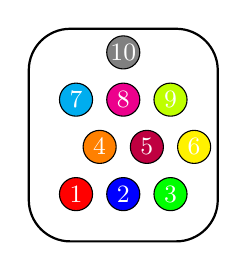
\begin{tikzpicture}[scale=0.6, every node/.style={font=\small, white}]
% Jar outline
\draw[thick, rounded corners=15pt] (0,0) rectangle (4,4.5);

% Balls (10 different colors + numbers)
\foreach \x/\y/\c/\n in {
  1/1/red/1,
  2/1/blue/2,
  3/1/green/3,
  1.5/2/orange/4,
  2.5/2/purple/5,
  3.5/2/yellow/6,
  1/3/cyan/7,
  2/3/magenta/8,
  3/3/lime/9,
  2/4/gray/10
} {
  % fill and draw circle
  \fill[\c] (\x,\y) circle (0.35);
  \draw (\x,\y) circle (0.35);
  % number on the ball
  \node at (\x,\y) {\n};
}
\end{tikzpicture}
\end{center}

\pause 
\colorbox{green!30}{\textbf{Solution.}} The number of possible sequences if we draw $k=6$ balls from the jar of $n=10$ balls and record the sequence in which they appear is:
%
\begin{align*}
= \begin{cases}
 10^6, & \text{if repetitions are permitted} \\
 (10)_6 = 10 \cdot 9 \cdot 8 \cdot 7 \cdot 6 \cdot 5, & \text{if repetitions are forbidden}	
 \end{cases}
\end{align*}

\end{frame}


\begin{frame}{Counting lists: Drawing items from a fixed pool}

\begin{mygreenbox}[title= Theorem 8.6 from Scheinerman]
The number of lists of length $k$ whose elements are chosen from a pool of $n$ elements 
%
\begin{align*}
= \begin{cases}
 n^k, & \text{if repetitions are permitted} \\
 (n)_k, & \text{if repetitions are forbidden}	
 \end{cases}
\end{align*}
\end{mygreenbox}

\pause \vfill 

\colorbox{red!30}{\textbf{Notation.}} The expression
\[  (n)_k \defeq \explaintermbrace{$k$ terms}{n \times (n-1) \times \cdots \times (n-k+1)}\]

is called a \textbf{falling factorial} and is read as \qq{$n$ falling $k$}.

%\pause \vfill 
%
%\colorbox{green!30}{\textbf{Solution to Lottery Problem.}} The number of possible sequences if we draw $k=6$ balls from the jar of $n=10$ balls and record the sequence in which they appear is:
%%
%\begin{align*}
%= \begin{cases}
% 10^6, & \text{if repetitions are permitted} \\
% (10)_6 = 10 \cdot 9 \cdot 8 \cdot 7 \cdot 6 \cdot 5, & \text{if repetitions are forbidden}	
% \end{cases}
%\end{align*}

\end{frame}



\begin{frame}{Practice Reading Quiz}

 \begin{myredbox}[title=Practice Reading Quiz (Lists)]
Five students in our class are randomly selected to form an emergency rock band.  The rock band will have a singer, a guitarist, a bassist, a drummer, and a keyboardist.  How many different rock bands can be formed in this way?  
\vfill
Notes: (1) Our class has 39 students. (2) If different students play different instruments, it counts as a "different band".
\end{myredbox}
\vfill
\pause 



 \begin{mygreenbox}[title=Solutions]

Let $N$ be the number of rock bands that can be formed.

\begin{enumerate}
	\item Suppose repetitions are permitted.  That is, one student can play multiple instruments.  Then \pause $N=39^5$. \pause 
	\item Suppose repetitions are forbidden. That is, no student plays more than one instrument (singing counts as an instrument).    Then \pause $N=(39)_5 = 39 \times 38 \times 37 \times 36 \times 35$.
\end{enumerate}

\end{mygreenbox}

\end{frame}


%\begin{frame}{Monday's Reading Quiz on Induction}
%
%\begin{myredbox}[title=Scoring rubric]
%\begin{tabularx}{\textwidth}{|X|L{1cm}|}
%\hline 
%\textbf{Description} & \textbf{E.C.} \\
%\hline 
%Correct and well-written. & +20\% \\
% Good work but some mathematical or writing errors that need addressing. & +15\%\\
%Some good intuition (about induction), but there is at least one serious flaw. & +5\%  \\
%I don't understand this, but I see that you did work on it. & +0\%  \\
%No work is evident.	&+0\% \\
%\hline
%\end{tabularx}
%\end{myredbox}
%\end{frame}
%
%
%\begin{frame}[standout]
%Review Induction Group Exercises.
%	
%\end{frame}


\begin{frame}{Why should computer scientists care about counting lists?}
\footnotesize

\begin{evidence}[blue]
\textbf{The multiplication principle is running time.}
Nested loops over $n$ and $m$ items run $n \cdot m$ times.%; a $k$-variable truth table has $2^k$ rows.
\end{evidence}

\pause
\begin{evidence}[orange]
\textbf{$n^k$ is the size of a key space.}
At $10^{10}$ guesses/s, 8 lowercase letters ($26^8$) fall in \alert{21 seconds};
12 printable characters ($95^{12}$) take \alert{1.7 million years}.
\end{evidence}

\pause
\begin{evidence}[red]
\textbf{Hash collisions use both formulas.}
If $k$ items each get one of $n$ random values, $P(\text{no repeats}) = (n)_k / n^k$.
So 23 people share a birthday with probability \alert{50.7\%}, and a 32-bit hash
collides after $\approx$\alert{77,000} items.
\end{evidence}

\pause
\begin{evidence}[green]
\textbf{Machine learning.}
Grid search over $5 \times 4 \times 3$ settings means \alert{60} training runs.
Bootstrap: \emph{with} replacement ($n^k$).  Train/test split: \emph{without} ($(n)_k$).
\end{evidence}

\pause
{\centering The skill: \textbf{does order matter, and are repeats allowed?}\par}

\end{frame}


\end{document}
